% !TeX encoding = UTF-8
% !TeX spellcheck = es_ES
% !TeX root = ../Thermal.tex
%!TEX root=../Thermal.tex

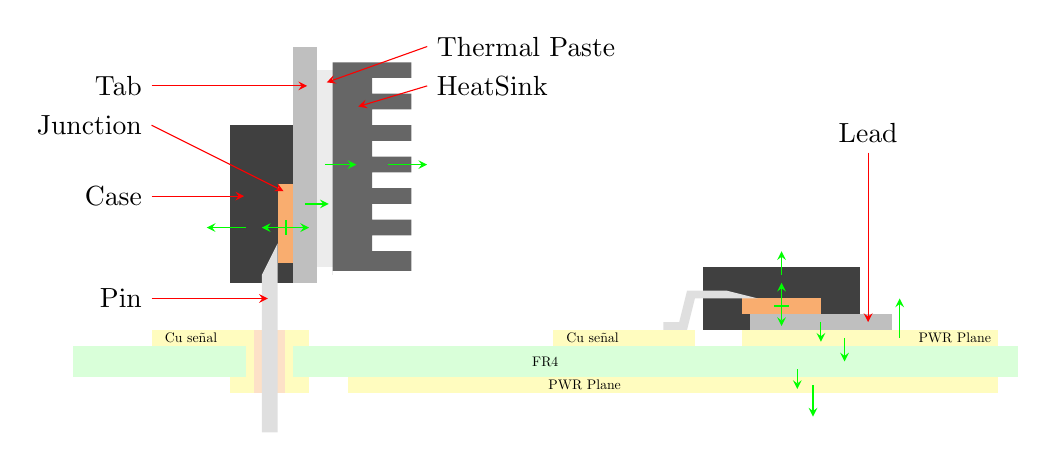
\begin{tikzpicture}[]

	\draw[draw=none,fill=green!15] (-6,-.2) rectangle +(12,.4);
	\draw[draw=none, fill=yellow!25] (-5,0.2) rectangle +(2,.2);
	\draw[draw=none, fill=yellow!25] (-2.5,-0.4) rectangle +(8.25,0.2);

	\node[scale=0.5] at(0,0){FR4};
	\node[scale=0.5] at (-4.5,.3){Cu señal};
	\node[scale=0.5] at (0.5,-.3){PWR Plane};
	\begin{scope}[shift={(-1,0)}]
		% TO-220
		\draw[draw=none,fill=black!75] (-3,1) rectangle +(.8,2);
		\draw[draw=none,fill=gray!50] (-2.2,1) rectangle + (0.3,3);
		\draw[draw=none, fill=Apricot] (-2.4,1.25) rectangle +(.2,1);
		\draw[draw=none,fill=gray!15] (-1.9,1.2) rectangle +(0.2,2.5);
		\draw[draw=none,fill=black!60](-1.7,1.1) -- ++(0,2.7)
		-- ++(1,0) -- ++(0,-.2) -- ++(-0.5,0) -- ++(0,-0.2)
		-- ++(0.5,0) -- ++(0,-.2) -- ++(-0.5,0) -- ++(0,-0.2)
		-- ++(0.5,0) -- ++(0,-.2) -- ++(-0.5,0) -- ++(0,-0.2)
		-- ++(0.5,0) -- ++(0,-.2) -- ++(-0.5,0) -- ++(0,-0.2)
		-- ++(0.5,0) -- ++(0,-.2) -- ++(-0.5,0) -- ++(0,-0.2)
		-- ++(0.5,0) -- ++(0,-.2) -- ++(-0.5,0) -- ++(0,-0.2)
		-- ++(0.5,0) -- ++(0,-.25) -- ++(-1,0);
		\draw[draw=none,fill=yellow!25] (-2.3,-0.4) rectangle +(0.1,0.6);
		\draw[draw=none,fill=yellow!25] (-2.8,-0.4) rectangle +(0.1,0.6);
		\draw[draw=none,fill=yellow!25] (-3,-0.4) rectangle +(1,0.2);
		\draw[draw=none,fill=Apricot!35] (-2.7,-.4) rectangle +(0.4,0.8);
		\draw[draw=none, fill=gray!25] (-2.4,1.5) -- ++(-.2,-.4) -- ++(0,-2) -- ++(0.2,0) -- ++(0,2.4);
		
		\node(th-J) at (-2.2,2.1){};
		\node(th-Tab) at (-1.9,3.5){};
		\node(th-Case) at (-2.7,2.1){};
		\node(th-Pin) at (-2.4,0.8){};

		\node(th-Tp) at (-1.9,3.5){};
		\node(th-HS) at (-1.5,3.2){};
		
		\draw[green,|-stealth] (-2.3,1.7) -- ++(0.3,0);
		\draw[green,-stealth] (-2.05,2) -- ++(0.3,0);
		\draw[green,-stealth] (-1.8,2.5) -- ++(0.4,0);
		\draw[green,-stealth] (-1.,2.5) -- ++(.5,0);

		\draw[green,-stealth] (-2.3,1.7) -- ++(-0.3,0);
		\draw[green,-stealth] (-2.8,1.7) -- ++(-0.5,0);
		

	\end{scope}
	\begin{scope}[shift={(3,.4)}]
		\draw[draw=none,fill=black!75] (-1,0) rectangle +(2,.8);
		\draw[draw=none,fill=gray!50] (-.4,0) rectangle +(1.8,.2);

		\draw[draw=none, fill=Apricot] (-0.5,.2) rectangle +(1,.2);
		\draw[draw=none, fill=gray!25] (-0.3,.4) -- ++(-.4,0.1)
		-- ++(-.5,0) -- ++(-.1,-.4) -- ++(-.2,0) -- ++(0,-.1)
		-- ++(.3,0) -- ++(.1,.4) -- ++(0.8,0);
		\draw [draw=none, fill=yellow!25] (-2.9,0) rectangle +(1.8,-0.2);
		\draw [draw=none, fill=yellow!25] (-0.5,0) rectangle +(3.25,-0.2);
		\node[scale=0.5] at (-2.4,-.1){Cu señal};
		\node[scale=0.5] at (2.2,-.1){PWR Plane};

		\draw[green, |-stealth] (-0,0.3) -- ++(0,0.3);
		\draw[green,-stealth] (0,0.7) -- ++(0,0.3);
		\draw[green, |-stealth] (-0,0.3) -- ++(0,0-.25);
		\draw[green,-stealth] (0.5,0.1) -- ++(0,-0.25);
		\draw[green,-stealth] (0.8,-0.1) -- ++(0,-0.3);
		\draw[green,-stealth] (1.5,-0.1) -- ++(0,0.5);
		\draw[green,-stealth] (0.2,-0.5) -- ++(0,-0.25);
		\draw[green,-stealth] (0.4,-0.7) -- ++(0,-0.4);

		\node(txt-lead) at(1.1,2.5) {Lead};
		\draw[red,-stealth] (txt-lead.south) -- (1.1,0.1);
	\end{scope}

	\node[left](txt-th-J) at (-5,3)  {Junction};
	\node[left](txt-th-Tab) at (-5,3.5)  {Tab};
	\node[left](txt-th-Case) at (-5,2.1)  {Case};
	\node[left](txt-th-Pin) at (-5,0.8)  {Pin};

	\draw[red,-stealth] (txt-th-J.east)-- (th-J);
	\draw[red,-stealth] (txt-th-Tab.east)-- (th-Tab);
	\draw[red,-stealth] (txt-th-Case.east)-- (th-Case);
	\draw[red,-stealth] (txt-th-Pin.east)-- (th-Pin);


	\node[right](txt-th-Tp) at (-1.5,4)  {Thermal Paste};
	\node[right](txt-th-HS) at (-1.5,3.5)  {HeatSink};
	\draw[red,-stealth] (txt-th-Tp.west)-- (th-Tp);
	\draw[red,-stealth] (txt-th-HS.west)-- (th-HS);
\end{tikzpicture}